% Compact journal version for IEEE Journal of Biomedical and Health Informatics (IEEEtran, two-column).
% The full preprint is main.tex; numbers here are taken from it unchanged.
\documentclass[journal]{IEEEtran}
\usepackage{amsmath,amssymb}
\usepackage{graphicx}
\usepackage{booktabs}
\usepackage{array}
\newcolumntype{L}[1]{>{\raggedright\arraybackslash}p{#1}}
\usepackage{cite}
\usepackage{url}
\usepackage[hidelinks]{hyperref}

\newtheorem{proposition}{Proposition}
\newtheorem{theorem}{Theorem}
\newtheorem{assumption}{Assumption}
\newtheorem{remark}{Remark}
\newcommand{\Prb}{\mathbb{P}}
\newcommand{\E}{\mathbb{E}}

\begin{document}
\title{Certified Adaptive Examination of Peripheral Blood Smears: When Information-Gain Stopping Fails, and What Can Be Guaranteed Instead}
\author{Qudrat~Ullah%
\thanks{Q. Ullah is with the Faculty of Informatics, University of Debrecen, Debrecen, Hungary (e-mail: qudratafridi@mailbox.unideb.hu). This work was supervised by Dr.\ Bal\'azs Harangi.}}
\markboth{IEEE Journal of Biomedical and Health Informatics}{Ullah: Certified Adaptive Examination of Peripheral Blood Smears}
\maketitle

\begin{abstract}
Automated examination of blood smears increasingly decides which fields to inspect and when to stop. We ask what it can guarantee about unexamined material, using pre-registered simulations from 28,280 expert-labelled cells, two external datasets and annotated bone-marrow regions from 99 patients. First, information-saturation stopping, reimplemented from InfoDPP-PAC, barely changed its stopping point with the rarity of decision-changing evidence; with one critical field among 200 ten-cell fields it missed 76\% of positive specimens (uniform sampling of equal size: 85\%). Second, without location information, any strategy must examine 95\% of the fields to certify at a 5\% error level that rare evidence is absent. Third, design-based, anytime-valid tests can certify that the blast proportion exceeds a 10\% or 20\% threshold, at a cost in verified cells governed mainly by the margin; near the threshold a 200-cell count was wrong in up to 27\% of specimens, whereas valid procedures were mostly undetermined. Fourth, validity held under acquisition shifts that cut blast sensitivity from 0.91 to 0.63 and 0.34, but efficiency did not: against uniform sampling with ALPHA, classifier-driven sampling needed 0.45--0.75 times the verified cells in distribution and, at margins of 0.05--0.10, 1.3--3.0 times under shift, and a 50\% uniform mixture at most 1.15 times (exploratory). Analysing cells of sampled fields as independent draws exceeded the nominal error in 27 of 75 real specimens, and single-reader verification certified that reader's count. Validity depends on the design, the unit of analysis and weighting, and verification.
\end{abstract}

\begin{IEEEkeywords}
Adaptive sampling, anytime-valid inference, blast count, blood smear, risk-limiting audit, sequential testing.
\end{IEEEkeywords}

\section{Introduction}
\IEEEPARstart{A}{} peripheral blood smear contains far more cells than any examiner inspects. A manual differential counts 100 or 200 leukocytes, and the variability this implies has long been known \cite{rumke1978}. Automated systems add a degree of freedom: they choose which fields to examine and when to stop. For questions that hinge on rare cells, such as the blast proportion relative to a classification threshold \cite{khoury2022who,arber2022icc}, what matters is not classifier accuracy on the examined fields but what can be said about the fields that were not examined.

Stopping rules based on \emph{information saturation} answer this implicitly, stopping when further fields would add little information about the selector's representation of the specimen. InfoDPP-PAC \cite{mittal2026infodpp} is a carefully constructed recent instance for whole-slide histopathology; its authors state that its certificate bounds residual information in the selection objective, not diagnostic performance, and that distinction is our starting point. We ask four questions. RQ1: does information-saturation stopping fail systematically when decision-changing evidence is rare? RQ2: why does certifying the \emph{absence} of rare evidence require near-exhaustive examination? RQ3: how many cells must be examined to certify a threshold decision under adaptive sampling? RQ4: where do the assumptions of anytime-valid audit methods break on real data?

Our contributions are:
\begin{itemize}
\item a pre-registered evaluation showing that, in the tested settings, the stopping point of saturation stopping barely changed with rarity, that its halting signal decoupled from critical evidence as cells were pooled into fields, and that on real marrow tiles it did worse than uniform sampling in low-blast specimens (RQ1);
\item a minimax lower bound showing that near-exhaustive examination is required of \emph{every} strategy without location information, its consequence for halting rules that ignore verified labels, and a proposition that ties a relevance-ranked search to the model's ROC curve (RQ2);
\item an evaluation of design-based, anytime-valid certification of blast-proportion assertions \cite{stark2023alpha,shekhar2023rlfa}: validity, cost from 500 to 4,000 cells against the best valid uniform design, and decisions at fixed budgets (RQ3);
\item an empirical examination of the assumptions behind these guarantees (RQ4) under acquisition shift on two external sources, spatial clustering, unequal field sizes and reader disagreement measured on real marrow annotations.
\end{itemize}
This is a methodological study. Most specimens are composites of real single-cell images, and no result establishes clinical diagnostic validity.

\section{Related Work}
R\"umke characterised the binomial and finite-population variability of manual differentials \cite{rumke1978}; for absence of rare events, the ``rule of three'' bounds a rate after zero events \cite{hanley1983}, and Proposition~\ref{prop:uniform} is its design-based finite-population counterpart. InfoDPP-PAC \cite{mittal2026infodpp}, a recent preprint, selects patches greedily under a blended information-gain and relevance objective and stops when the largest information gain among unselected patches falls below a concentration-corrected threshold. Its certificate rests on a stability assumption whose constant and target are assumed rather than derived; our results do not depend on it. Blast recognition itself is well studied \cite{matek2019aml}; our question concerns examination and inference.

Risk-limiting audits bound the probability of confirming a false assertion about a finite population \cite{lindeman2012gentle}. ALPHA \cite{stark2023alpha} turns assertions into bounded-mean tests through an \emph{assorter}, with a test supermartingale for sampling without replacement \cite{waudbysmith2020wor,waudbysmith2024betting,ville1939}; Shekhar et al.\ \cite{shekhar2023rlfa} extend this to weighted, adaptive sampling with side information, and stratified extensions exist \cite{spertus2024stratified}. Prediction-powered inference \cite{angelopoulos2023ppi}, prediction-powered e-values \cite{csillag2025ppe} and active inference \cite{zrnic2024active} combine predictions with a verified subset, mostly as fixed-sample statements about a superpopulation; our tests are anytime-valid statements about one finite specimen. Two failures we measure are textbook survey sampling, the design effect of cluster sampling \cite{kish1965} and the bias of the mean-of-ratios estimator \cite{cochran1977}, and classifier-driven sampling is probability-proportional-to-size sampling \cite{hansen1943,horvitz1952}; their size on real smear arrangements, and their effect on anytime-valid certificates, are not known.

\section{Setting and Theory}
\subsection{Estimands}
A specimen has $N$ fields; field $i$ holds $m_i$ cells, $B_i$ of them blasts, $M=\sum_i m_i$, and $p=\sum_iB_i/M$. We distinguish \emph{detection} (has a critical field, one with at least one blast, been examined?), \emph{estimation} of $p$, and \emph{threshold certification} ($p>\theta$?). We use $\theta=0.10$, the blast percentage at which the International Consensus Classification (2022) separates myelodysplastic syndrome with excess blasts from MDS/AML \cite{arber2022icc}, and $\theta=0.20$, the WHO 5th-edition threshold for acute myeloid leukemia without defining genetic abnormalities \cite{khoury2022who}. Both count blast equivalents, which our labels do not; the thresholds are analysed separately and are inputs to a procedure, not validated here. An examiner selects fields sequentially, possibly using features $x$ and past labels, and a selected field is \emph{verified}: its cells' labels are revealed. All probabilities are over the examiner's randomisation for a fixed specimen, so the guarantees are finite-population and design-based. They concern the sampling frame, the fields the imaging system can present; which cells an analyser images and how the smear relates to the patient's blood are outside it.

\subsection{Certifying absence (RQ2)}
Let $C$ be the set of $k$ critical fields and $M_n$ the event that none is among $n$ examined fields; let $h(N,k,n)=\binom{N-k}{n}/\binom{N}{n}$.
\begin{proposition}[Uniform sampling]\label{prop:uniform}
Under sampling of $n$ fields without replacement, $\Prb(M_n\mid C)=h(N,k,n)$; for $k=1$ this is $1-n/N$, so $\Prb(M_n)\le\alpha$ iff $n\ge\lceil(1-\alpha)N\rceil$. For $0\le n\le N$, $[\max\{0,1-n/(N-k+1)\}]^k\le h\le(1-n/N)^k$, so $n\ge N(1-\alpha^{1/k})$ suffices.
\end{proposition}
\begin{assumption}[No location information]\label{ass:A}
The class of specimens regarded as possible, given the observed features $x$, contains every placement $C$ with $|C|=k$.
\end{assumption}
\begin{theorem}[Minimax lower bound]\label{thm:minimax}
Under Assumption~\ref{ass:A}, every policy, adaptive or not, randomised or not, that examines at most $n$ fields satisfies $\max_{|C|=k}\Prb_\pi(M_n\mid x,C)\ge h(N,k,n)$. Uniform sampling attains the bound; every deterministic policy has worst-case miss probability $1$ if $n\le N-k$.
\end{theorem}
\emph{Proof.} Fix $x$ and a realisation $u$ of the examiner's randomness. On the run in which every examined field is negative, every input to the policy is determined by $(x,u)$, so it examines a fixed set $A(u)$, $|A(u)|\le n$, and the actual run misses $C$ iff $C\cap A(u)=\emptyset$; hence $\Prb_\pi(M_n\mid x,C)=\Prb_U(C\cap A(U)=\emptyset)$. Let $C$ be uniform over $k$-subsets, independent of $U$, which Assumption~\ref{ass:A} permits. For fixed $u$ the fraction of $k$-subsets disjoint from $A(u)$ is at least $\binom{N-n}{k}/\binom{N}{k}=h(N,k,n)$; averaging over $U$, and noting that the maximum over $C$ is at least the average, gives the bound (Yao's principle \cite{yao1977}). Uniform sampling attains it by Proposition~\ref{prop:uniform}; a deterministic policy examines one set $A$ with $|A|\le N-k$, and placing $C$ outside it gives miss probability 1.\hfill$\square$

We verified all statements exactly in rational arithmetic and, for $N\le7$, by solving the search game as a linear program. If $k$ is unknown, the worst case is $k=1$, so certifying absence at level $\alpha$ needs $\lceil(1-\alpha)N\rceil$ fields (Fig.~\ref{fig:partII}). The theorem also bears on RQ1: a rule whose halting depends only on the features and its own randomisation, not on verified labels, examines a number of fields fixed before any evidence is seen, so with one critical field its worst-case miss probability is at least $1-\bar n/N$ when it examines $\bar n$ fields on average. If verification misses an examined critical field with probability $\beta$, absence cannot be certified below $\beta$ even by a census.

Informative features can let a search beat the bound on average, through a model of where evidence lies:
\begin{proposition}[Ranked search]\label{prop:bridge}
Let one field be critical with score $S_c\sim F_1$, and the other $N-1$ scores be independent with distribution $F_0$. A scan of the $n$ highest-scoring fields misses the critical field with probability $\E_{S_c}[\Prb(\mathrm{Bin}(N-1,1-F_0(S_c))\ge n)]$, which tends to $1-\mathrm{TPR}(t_r)$ as $N\to\infty$ with $n/(N-1)\to r$, where $t_r$ is the threshold with false-positive rate $r$ and $F_0$ is continuous and strictly increasing at $t_r$.
\end{proposition}
Given $S_c=s$, the critical field is missed iff at least $n$ others score above $s$; the limit follows by dominated convergence. With $F_1=F_0$ the formula returns $1-n/N$. Certifying absence by ranking thus needs a sensitivity of about $1-\alpha$ at a false-positive rate of $n/N$, a property of the model that no sampling design supplies. It is an average-case result under independence, neither a proof that only ranking helps nor a worst-case guarantee: a ranked scan surely misses a critical field placed among low-scoring fields.

\begin{figure}[t]
\centering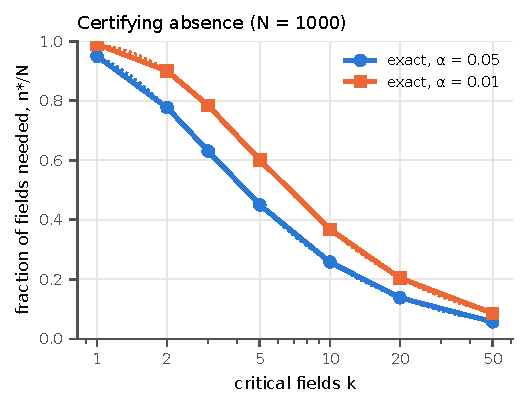
\includegraphics[width=0.86\columnwidth]{figures/fig2_partII.pdf}
\caption{Fraction of fields that any strategy without location information must examine to certify the absence of $k$ critical fields ($N=1000$; exact values solid, sufficient closed form $1-\alpha^{1/k}$ dotted).}\label{fig:partII}
\end{figure}

\subsection{Certifying a threshold assertion (RQ3)}
Making ``$p>\theta$'' true requires more than $\theta M$ blasts, which cannot hide in one field, so the bound above does not apply. With equal field sizes and the assorter $a_j=b_j/(2\theta)$, $b_j$ being the blast fraction of the $j$-th sampled field, $\bar a>1/2\iff p>\theta$, a one-sided bounded-mean assertion. Under uniform sampling of fields, ALPHA \cite{stark2023alpha} gives a test supermartingale; rejecting when it exceeds $1/\alpha$ controls false certification at $\alpha$ at any data-dependent stopping time. For adaptive sampling, write $p=\sum_iw_if_i$ with known weights and $f_i\in[0,1]$. If the field $I_t$ is drawn from a predictable distribution $q_t$, the observation $Z_t=w_{I_t}f_{I_t}/q_t(I_t)$ has conditional mean equal to the unsampled mass, which under $H_0:p\le\theta$ is at most $\mu_t=\theta-\sum_{s<t}w_{I_s}f_{I_s}$; a betting process $\prod_s(1+\lambda_s(Z_s-\mu_s))$ with predictable bets $0\le\lambda_s\le1/\mu_s$ is a test supermartingale whatever the classifier does \cite{shekhar2023rlfa}. We use their prop-MS sampler, $q_t(i)\propto w_iS_i$ with a floor ($S_i$ the field's mean classifier score), with approximate-Kelly bets and, exploratorily, hedged bets (the average of the processes with $\lambda_s=\kappa/\mu_s$, $\kappa\in\{0.05,0.1,0.2,\dots,0.9\}$). Validity requires only known $q_t$ and verified labels; positivity of $q_t$ is needed for power and for ``$p<\theta$'' certificates, not for validity of ``$p>\theta$'', because $f_i\ge0$.

Averaging field proportions, however, estimates $N^{-1}\sum_iB_i/m_i$, which is not $p$ when field sizes differ.
\begin{proposition}[Unequal field sizes]\label{prop:unequal}
(a) If every $m_i$ is known, $w_i=m_i/M$ and $f_i=B_i/m_i$ give $\sum_iw_if_i=p$, so the weighted test is valid for $H_0:p\le\theta$. (b) If only $m_i\le m_{\max}$ is known, $a_i=(B_i-\theta m_i+\theta m_{\max})/m_{\max}\in[0,1]$ and $N^{-1}\sum_ia_i>\theta\iff p>\theta$, so equal-weight tests on $a_i$ with null mean $\theta$ are valid.
\end{proposition}
For (b), $0\le B_i\le m_i\le m_{\max}$ bounds $a_i$, and $\sum_ia_i=(\sum_iB_i-\theta M)/m_{\max}+N\theta$. The margin shrinks by $\bar m/m_{\max}$, so a loose bound costs power.
\begin{remark}[Imperfect verification]\label{rem:verif}
Suppose the verifier counts the same $M$ cells as the reference and, in this specimen, its false blast calls number at most $\beta_0$ times the true non-blasts. Then $\tilde p\le p+\beta_0(1-p)$, so testing $\tilde p>\theta+\beta_0(1-\theta)$ is valid for $p>\theta$; symmetrically, testing $\tilde p<\theta(1-\beta_1)$ is valid for $p<\theta$ if missed blasts number at most $\beta_1$ times the true blasts. These are per-specimen bounds that no design supplies; average disagreement rates are not such bounds, and excluding cells the reference counts can raise $\tilde p$ without any false blast call.
\end{remark}

We compare, on the same specimen, ALPHA and betting with uniform sampling; betting with classifier-driven sampling, with and without a control variate; an invalid \emph{uncorrected} design that ranks fields by score but analyses them as uniform draws; and conventional 100- and 200-cell counts. Uniform ALPHA, the best valid design without a classifier in our runs, is the reference for cost ratios.


\section{Experimental Design}
\subsection{Pre-registration and status of analyses}
Hypotheses, decision rules, seeds and scripts were frozen in five git tags, each pushed before the corresponding data were generated; first confirmatory outputs followed the push by 43\,s to 18\,min (audit table in the repository). ``Confirmatory'' means fresh Monte Carlo draws on a disjoint seed family over the same cell pool, which protects against analytic flexibility but not against effects specific to that pool; only H4a--c and H7a used data not analysed before. All later analyses, including a rerun of all cost comparisons on the same specimens for the three cell sources (seed family 20261101), used new seed families and are labelled exploratory; all deviations are logged in the repository.

\subsection{Data}
\emph{KU-Optofil} \cite{yarikan2026kuoptofil}: Sysmex DI-60 images of May--Gr\"unwald--Giemsa peripheral blood smears labelled by haematologists; we used 28,280 cells from 275 identified patients (13 classes) in five patient-grouped folds. Blasts come from only 11 patients (489 blasts). \emph{RV-PBS} \cite{rvpbs2024}: 752 annotated cells (153 blasts) from phone-camera fields, used only as an acquisition-shift probe. \emph{MLL23} \cite{shetabboushehri2025mll23}: 41,621 peripheral-blood cells (Pappenheim stain, Metafer scanner), 8,606 myeloblasts; we excluded atypical promyelocytes (blast equivalents our labels do not count), smudge cells and normoblasts, leaving 36,529; there are no patient identifiers. \emph{BoneMarrowWSI} \cite{hofener2025bmwsi,hofener2025descriptor}: pediatric bone-marrow aspirate slides with 228 exhaustively annotated regions of about $225\,\mu$m; we used the annotations, the per-round reader labels, and the image pixels of the annotated regions.

\subsection{Representation, teachers and specimens}
Cells were embedded with a frozen DINOv2 ViT-S/14 \cite{oquab2023dinov2}; a logistic probe cross-fitted by patient fold reached an out-of-fold AUC of 0.979. The pre-registered \emph{cell-level teacher} scores a field by its largest cell score, which presupposes cell detection; an exploratory \emph{field-level teacher} is a logistic regression on the pooled field embedding, the representation the selector sees. Part~I composites have $N=200$ fields of $m\in\{1,5,10,20\}$ cells (mean-pooled embeddings) with $k\in\{1,2,5,10,20\}$ critical fields of one blast. Part~III composites have 100 fields of 5 cells ($M=500$) with $p$ fixed exactly, blasts from all 489 blasts and background cells from blast-free patients; 10\% of that background are platelets and erythroblasts, so $p$ is the blast share of imaged objects (a leukocyte-only background changed nothing material). Exploratory extensions use $M$ up to 4,000 and field sizes drawn from BoneMarrowWSI.

\subsection{InfoDPP-PAC and baselines}
No code has been released. We implemented the objective, greedy blended gain and halting rule (Eqs.~3--7 of \cite{mittal2026infodpp}) with the published weights, set $\rho=1$, and calibrated $\tau$ on blast-free specimens of other folds so that the median stop is 16.3\% of all fields. The original runs stopped at 16.3\% of a 300-patch budget, about 2.4\% of a slide (a ratio of reported averages, not the original configuration), so our setting gives InfoDPP-PAC about seven times its own examination share; we also report a 2.4\% run. A random seed of 5 fields fits the Gaussian process and is not counted as examined. Baselines were uniform sampling at the same per-episode cost (paired), a fixed field order, confidence-based stopping (stop at the first field with relevance $\ge0.9$ or after 30 consecutive fields $\le0.1$), and exhaustive examination.

\subsection{Statistics}
Miss-rate differences are reported with $t$ intervals on the five patient-grouped folds: episodes resample cells from one pool of 275 patients (blasts from 11), so the pre-registered exact McNemar tests on paired episodes measure Monte Carlo precision only. False certification: Clopper--Pearson intervals and one-sided exact binomial tests of rate $\le0.05$. Costs: paired Wilcoxon tests with Holm correction and ratios of medians with bootstrap intervals; real-data analyses bootstrap over patients; $\alpha=0.05$ unless stated. Validity claims rest on design-based theorems that hold for every specimen; miss rates and costs are estimates for this pool. Our ALPHA and betting statistics agree with the reference implementation (SHANGRLA) to within $3\times10^{-13}$ in log scale on 2,000 random cases, apart from a conservative rule missing from our frozen ALPHA that changed no median cost; a suite of 50 deterministic tests, with adversarial samplers and negative controls, is in the repository.

\section{Results}
\subsection{Information-saturation stopping (RQ1)}\label{sec:partI}
In 24,000 confirmatory episodes the median stop was 32--33 of 200 fields in every cell, varying by at most one field across rarity levels (H1a). This is an empirical finding: the halting statistic has no relevance term but depends on the embeddings and the selected set. The AUC with which the information-gain term separates critical from non-critical fields fell from 0.778 at $m=1$ to 0.593, 0.552 and 0.525 at $m=5,10,20$, whereas the field-level teacher on the same pooled embeddings kept 0.978, 0.925, 0.882 and 0.827 (Kill-test 1; the pre-registered cell-level teacher gave 0.977--0.896). The evidence survives pooling; the halting signal does not use it.

At $k=1$, InfoDPP-PAC missed the critical field in 0.315, 0.681, 0.759 and 0.805 of specimens at $m=1,5,10,20$; uniform sampling of the same size missed 0.822, 0.830, 0.846 and 0.828, matching $1-n/N$ (H1d; Fig.~\ref{fig:partI}). The advantage shrank with dilution for every $k$ (H1b), but the pre-registered claim of no advantage at $m\ge10$ failed (H1c): the difference was $-0.087$ at $m=10$ (fold-level $t$ interval $[-0.153,-0.021]$; pre-registered episode-level interval $[-0.107,-0.067]$) and $-0.023$ $[-0.050,0.003]$ at $m=20$. Dilution, not rarity, governed the gap; rarity drove the absolute miss rate of every method.

Two other saturation rules, pure information-gain sampling and $k$-center coverage stopping, calibrated to the same cost on 4,000 new specimens, missed within 0.04 of InfoDPP-PAC in every cell. A scan ranked by the field-level teacher missed 0.05, 0.14, 0.21 and 0.37, against 0.051, 0.146, 0.221 and 0.394 predicted by Proposition~\ref{prop:bridge}: relevance, not the stopping criterion, separated the rules. At about 2.4\% of the specimen, InfoDPP-PAC made 4--5 selections after its seed; its advantage was $-0.17$ $[-0.27,-0.08]$ with single-cell fields and at most about 0.03 otherwise.

On real image tiles (exploratory; BoneMarrowWSI, 3,040 tiles of about $56\,\mu$m from 99 patients, specimens of 16--32 tiles, 200 runs each), InfoDPP-PAC stopped after 5.4 tiles on average. In the 24 specimens with at most a quarter of tiles critical it missed every critical tile in 0.80 of runs against 0.70 for uniform sampling ($+0.105$ $[0.002,0.203]$; worse in 18 of 24), and in at least 95\% of runs in 15 specimens, as Theorem~\ref{thm:minimax} predicts for a nearly deterministic selector.

\begin{figure*}[t]
\centering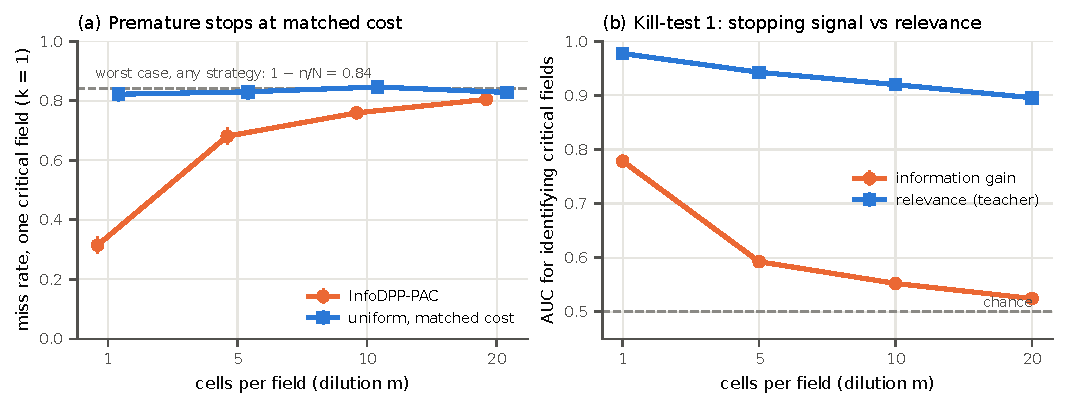
\includegraphics[width=0.76\textwidth]{figures/fig1_partI.pdf}
\caption{RQ1, confirmatory run. (a) Miss rate with one critical field for InfoDPP-PAC and for uniform sampling of the same size (95\% Wilson intervals); dashed: the worst-case bound $1-n/N$. (b) AUC of the information-gain term and of the cell-level teacher for ranking critical above non-critical fields; dashed, exploratory: the field-level teacher on the same pooled embeddings as the selector (10,000 separate episodes).}\label{fig:partI}
\end{figure*}

\subsection{Certified threshold decisions (RQ3)}
In 12,000 confirmatory 500-cell specimens, all four valid designs kept false certification at $p=\theta$ between 0.001 and 0.022 (H3a), whereas the uncorrected design certified falsely in 0.993 ($\theta=0.10$) and 0.889 ($\theta=0.20$) of boundary specimens (H3b; Fig.~\ref{fig:partIII}). Classifier-driven betting needed fewer cells than uniform ALPHA at every $p>\theta$ (H3c), 0.45--0.75 times as many, for example 75 vs.\ 165 at $p=0.15$, $\theta=0.10$, and cost fell with the margin (H3d). Uniform betting with approximate-Kelly bets needed 1.03--1.83 times the cells of ALPHA, so savings measured against it (0.28--0.73) are overstated; with hedged bets (exploratory, 4,400 specimens) it matched ALPHA (0.98--1.17), while classifier-driven medians changed by at most 14\%.

With specimens of up to 4,000 cells (exploratory; 17,600 specimens), false certification stayed $\le0.040$ at $\alpha=0.05$ and $\le0.007$ at $\alpha=0.01$, and cost was governed mainly by the margin: at $p=0.15$ against $\theta=0.10$, uniform ALPHA needed a median of 165, 205 and 245 cells at $M=500$, 1,000 and 4,000 and classifier-driven betting 80, 80 and 85. At margins of 0.05 or more and $M=4{,}000$, uniform ALPHA was within 20\% of Wald's approximation $\log(1/\alpha)/\mathrm{KL}(p\|\theta)$ \cite{wald1945}; within 0.02 of the threshold it still grew with $M$, to 1,583 ($\theta=0.10$) and 2,033 cells ($\theta=0.20$) at $M=4{,}000$, so the near-census at $M=500$ was a small-specimen effect. Savings count expert-verified cells; every field must still be imaged and scored. Lowering $\alpha$ to 0.01 multiplied the cost by 1.0--1.7; the claim that $\alpha=0.01$ is unattainable concerns conformal-risk-control calibration (negative risk budget below 99 positive episodes), not design-based tests.

At fixed budgets (exploratory; 2,000-cell specimens, cells sampled individually), we compared three-way decisions (``above'', ``below'', ``undetermined''; Table~\ref{tab:decision}). Within 0.02 of the threshold a 200-cell count, the usual peripheral-blood differential, was wrong in 11--27\% of specimens (100 cells: 18--37\%). Valid procedures, two one-sided sequential ALPHA tests or exact hypergeometric tests at $\alpha/2$ each, were wrong in at most 0.7\% of specimens off the threshold, but at those margins returned ``undetermined'' in 61--98\% of specimens at budgets up to 500 cells. With a budget fixed in advance and uniform sampling, a fixed-$n$ test is decisive more often; anytime validity pays when the examiner stops on the data or samples adaptively.

\begin{figure*}[t]
\centering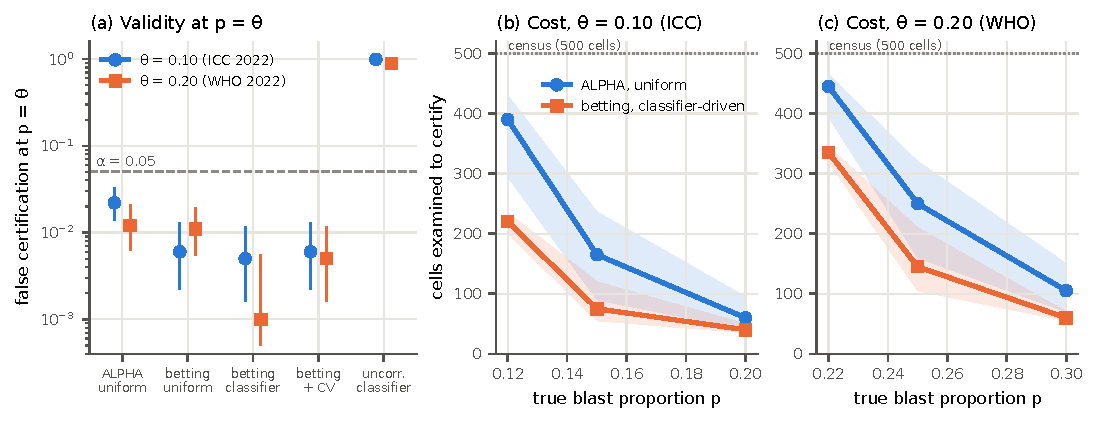
\includegraphics[width=0.76\textwidth]{figures/fig3_partIII.pdf}
\caption{RQ3, confirmatory run (500-cell specimens; $\alpha=0.05$). (a) False certification at $p=\theta$ with 95\% Clopper--Pearson intervals (log scale); CV: control variate; the uncorrected design analyses classifier-ranked fields as uniform draws. (b, c) Median cells to certification with interquartile bands; specimens that never certify count as 500 cells.}\label{fig:partIII}
\end{figure*}


\begin{table}[t]
\centering\footnotesize
\caption{Decisions after $n$ individually sampled cells (exploratory; $M=2{,}000$; 2,000 specimens per row). Conv.: share wrong for the conventional $n$-cell count; Exact (fixed-$n$ hypergeometric) and Seq.\ (sequential): share correct\,/\,wrong for valid tests at $\alpha/2$ per side; the rest is ``undetermined''; $\epsilon$: $<0.01$.}\label{tab:decision}
\setlength{\tabcolsep}{1.6pt}
\begin{tabular}{@{}llcccccc@{}}
\toprule
 & & \multicolumn{3}{c}{$n=200$} & \multicolumn{3}{c}{$n=500$}\\
\cmidrule(lr){3-5}\cmidrule(l){6-8}
$\theta$ & $p$ & Conv. & Exact & Seq. & Conv. & Exact & Seq.\\
\midrule
0.10 & 0.08 & 0.11 & 0.10/0 & 0.06/$\epsilon$ & 0.03 & 0.39/0 & 0.15/$\epsilon$\\
0.10 & 0.12 & 0.22 & 0.15/$\epsilon$ & 0.05/$\epsilon$ & 0.06 & 0.34/0 & 0.15/$\epsilon$\\
0.10 & 0.15 & 0.01 & 0.60/0 & 0.31/$\epsilon$ & 0.00 & 0.96/0 & 0.86/$\epsilon$\\
0.20 & 0.18 & 0.19 & 0.12/$\epsilon$ & 0.04/$\epsilon$ & 0.08 & 0.23/0 & 0.09/$\epsilon$\\
0.20 & 0.22 & 0.27 & 0.09/$\epsilon$ & 0.03/$\epsilon$ & 0.12 & 0.25/$\epsilon$ & 0.08/$\epsilon$\\
0.20 & 0.25 & 0.05 & 0.38/$\epsilon$ & 0.16/0 & 0.00 & 0.87/0 & 0.59/0\\
\bottomrule
\end{tabular}
\end{table}

\begin{figure*}[t]
\centering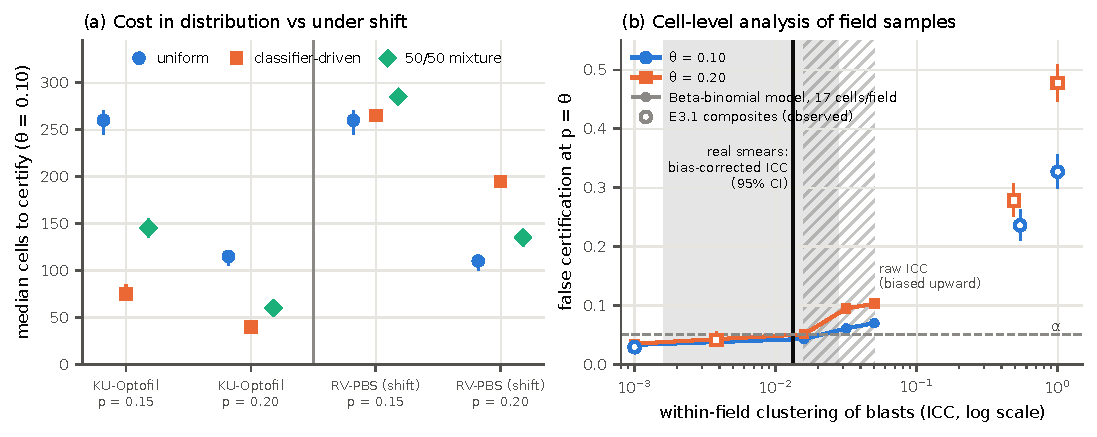
\includegraphics[width=0.76\textwidth]{figures/fig4_rq4.pdf}
\caption{RQ4. (a) Median cells to certify $p>0.10$ with 95\% bootstrap intervals, in distribution (KU-Optofil) and under two acquisition shifts (MLL23, RV-PBS): uniform ALPHA, classifier-driven betting and a 50\% mixture with hedged bets on the same specimens (exploratory rerun, 400 specimens per point); all designs kept false certification $\le0.034$. (b) False certification at $p=\theta$ when cells of sampled fields are analysed as individual draws: composites with scattered or clustered arrangements (markers) and a Beta-binomial model with 17 cells per field (lines). Solid band and line: bias-corrected clustering of real marrow regions (exploratory); hatched: the raw, upward-biased estimate, for comparison.}\label{fig:rq4}
\end{figure*}

\subsection{Where the assumptions break (RQ4)}\label{sec:rq4}
\emph{Classifier error.} On KU-Optofil, blast recall at 95\% specificity varied across the 11 blast patients from 0.39 to 1.00, false-positive rates across blast-free patients were overdispersed 6.6-fold, and errors concentrated in immature granulocytes and lymphoid cells. Certification stayed valid with blasts drawn only from low-recall patients ($\le0.007$), at 2.3 times the cost.

\emph{Acquisition shift.} Applied unchanged, the KU-trained probe's blast sensitivity fell to 0.340 [0.250, 0.421] on RV-PBS (H4a) and 0.63 [0.62, 0.64] on MLL23 (AUC 0.786 and 0.915), while its false-positive rate barely rose (0.058 and 0.060 against 0.050; H4b not supported). Every design stayed valid (H4c; all $\le0.034$), but efficiency did not transfer (Fig.~\ref{fig:rq4}a). Against uniform ALPHA on the same specimens (exploratory rerun), classifier-driven sampling needed 1.30 [1.18, 1.37] and 1.46 [1.36, 1.75] times the cells on MLL23 at $p=0.15$ and $0.20$, and 1.67 [1.53, 1.75] and 3.00 [2.79, 3.33] times on RV-PBS; the confirmatory comparison with uniform betting gave 1.77 on RV-PBS at $p=0.20$ (H6d). A 50\% uniform mixture stayed valid (H6a); with approximate-Kelly bets it kept 58--73\% of the saving over uniform betting (H6c) but cut the RV-PBS excess only to $+23\%$ [11, 30], missing the pre-registered 20\% bound (H6b); with hedged bets it needed 0.61--0.81 times the cells of ALPHA in distribution, 0.77--0.82 on MLL23 and 0.95--1.15 on RV-PBS (exploratory).

\emph{Spatial clustering and the unit of analysis.} Analysing the cells of sampled fields as independent draws ignores the design effect \cite{kish1965}: under strong synthetic clustering (18,000 specimens) it certified falsely in 0.327 ($\theta=0.10$) and 0.478 ($\theta=0.20$) of boundary specimens (H5b), whereas field-level designs stayed valid ($\le0.042$, H5a), although clustering doubled the cost of uniform field sampling (H5c). In 116 exhaustively annotated marrow regions of 75 patients, blasts were clustered (H7a; permutation $p=0.024$ at the quadrant and $0.0005$ at the $4\times4$ scale) but weakly: the bias-corrected intraclass correlation was 0.013 [0.002, 0.028] and 0.043 [0.018, 0.067] (exploratory), a design effect of about 1.2 for 5-cell fields, and a null-centred estimate of 0.059 [0.007, 0.108] at $4\times4$ in the 32 regions with at most 30\% blasts. We then used each patient's regions as a real specimen, with $4\times4$ subregions as fields and its own proportion as threshold (an exact null; 400 sampling orders per specimen; exploratory). The weighted test of Proposition~\ref{prop:unequal}(a) certified falsely in 0.001 of runs and at most 0.01 in any specimen; the cell-level analysis gave 0.051 overall, yet exceeded 0.05 in 27 of 75 specimens (21 significantly; up to 0.335), including 7 of the 23 with at most 20\% blasts. Validity is a statement about each specimen, and a pooled rate can hide failures. These specimens are small (median 105 cells) and mostly high-blast.

\emph{Unequal field sizes.} Marrow quadrants hold 12--29 nucleated cells (interquartile range). With these sizes, averaging field proportions, the mean-of-ratios estimator \cite{cochran1977}, certified falsely in 0.38 [0.35, 0.41] and 0.32 [0.29, 0.35] of boundary specimens even with blasts placed independently of size, and in every specimen with blasts enriched in small fields: the test is valid for the mean of proportions, which is the wrong quantity. Both constructions of Proposition~\ref{prop:unequal} stayed at or below 0.005; with known counts, classifier-driven sampling certified $p=0.15$ against $\theta=0.10$ with 297 cells against 646 for uniform sampling, and the bounded assorter needed 631 because $\bar m/m_{\max}\approx0.24$.

\emph{Verifier error.} BoneMarrowWSI publishes each reading round's labels, not who read which cell \cite{hofener2025bmwsi}. The second reader called a blast in 1.1\% [0.7, 1.7] of the first reader's counted non-blasts and a non-blast in 1.2\% [0.8, 1.6] of its blasts; 2.7\% of cells were counted by one reader only. With the first reader as verifier and the consensus as truth (83 specimens), the reader's proportion differed from the consensus by a median of 0.005 (maximum 0.075). Each specimen was tested at its own consensus proportion and examined almost completely, so the sign of the reader's error decided the outcome: ``$p>\theta_s$'' was certified falsely in all 23 specimens in which the reader over-counted (0.28 of runs), ``$p<\theta_s$'' in all 52 in which it under-counted (0.63), and in at most 0.008 of runs in the 8 without error. The test certified the reader's count, as designed. Remark~\ref{rem:verif} with average disagreement rates, which are not per-specimen bounds, did not repair this (0.16, 0.42); a margin of 0.03, selected on the same specimens, sufficed for ``above'' but not for ``below''.

\emph{One benchmark.} Table~\ref{tab:bench} puts these designs and conditions side by side: where their assumptions held, design-based tests kept false certification at or below 0.034, whereas every analysis without a design-based guarantee failed in some condition, even where it looked acceptable in distribution (cells as draws, 0.041) or pooled over real arrangements (0.051). Validity transferred across conditions; efficiency did not.

\begin{table*}[t]
\centering\footnotesize
\setlength{\tabcolsep}{4pt}
\caption{One benchmark across conditions (stored results; no new simulation). Top: share of specimens certifying ``$p>\theta$'' at $p=\theta$ ($\alpha=0.05$; larger of $\theta=0.10$, $0.20$; 400--1,000 specimens); BoneMarrowWSI: pooled over runs with $\theta_s=p_s$ [largest specimen rate]. Bottom: median cells to certify $p=0.15$ against $\theta=0.10$ (uncertified specimens count all cells). Specimens: 500 cells; about 1,300 with unequal fields; median 105 real cells. Stressed: assumption tested (unit: analysed unit = sampled unit; target: cell-weighted $p$). C/X: confirmatory/exploratory run. $^a$Unequal fields and BoneMarrowWSI: ALPHA on the bounded assorter, betting with known counts (Prop.~\ref{prop:unequal}). $^b$Coincides with ALPHA for equal fields; 1.00 with blasts enriched in small fields. $^c$Exploratory rerun, all designs on the same specimens; uniform ALPHA sees only labels. One reader with margin 0.03: 0.0003 [0.013].}\label{tab:bench}
\begin{tabular}{@{}l cccc cc cc@{}}
\toprule
 & \multicolumn{4}{c}{Composites of KU-Optofil cells} & \multicolumn{2}{c}{External cells} & \multicolumn{2}{c}{BoneMarrowWSI}\\
\cmidrule(lr){2-5}\cmidrule(lr){6-7}\cmidrule(l){8-9}
 & In distr. & Clustered & Confusable & Unequal & RV-PBS & MLL23 & Real & One\\
 & & & backgr. & fields & & & arrangem. & reader\\
\emph{Stressed} & --- & \emph{unit} & \emph{classifier} & \emph{target} & \multicolumn{2}{c}{\emph{classifier transfer}} & \emph{geometry} & \emph{verifier}\\
\emph{Status} & C & C & X & X & C & X & X & X\\
\midrule
\multicolumn{9}{@{}l}{\emph{False certification of ``$p>\theta$'' at $p=\theta$}}\\
ALPHA, uniform$^{a}$ & 0.022 & 0.025 & 0.031 & 0 & 0.026$^c$ & 0.034$^c$ & 0 [0] & ---\\
Betting, uniform$^{a}$ & 0.011 & 0.005 & 0.011 & 0.005 & 0.011 & 0.011 & 0.001 [0.010] & 0.277 [1.00]\\
Betting, classifier-driven & 0.005 & 0.003 & 0.007 & 0.001 & 0.001 & 0.001 & --- & ---\\
Betting, 50\% mixture & 0.014 & --- & --- & --- & 0.003 & 0.004 & --- & ---\\
Hedged betting, 50\% mixture$^c$ & 0.028 & --- & --- & --- & 0.025 & 0.030 & --- & ---\\
\addlinespace
Ranked, analysed as uniform & 0.993 & --- & --- & --- & --- & --- & --- & ---\\
Cells of fields as draws & 0.041 & 0.478 & --- & --- & --- & --- & 0.051 [0.335] & ---\\
Mean of field proportions$^{b}$ & --- & --- & --- & 0.379 & --- & --- & 0.062 [1.00] & ---\\
100-cell count, ``above'' & 0.427 & 0.388 & --- & --- & --- & --- & --- & ---\\
\midrule
\multicolumn{9}{@{}l}{\emph{Median cells to certify $p=0.15$ against $\theta=0.10$}}\\
ALPHA, uniform$^{a}$ & 165 & 345 & 160 & 1{,}031 & 165$^c$ & 165$^c$ & --- & ---\\
Betting, uniform$^{a}$ & 270 & 355 & 265 & 646 & 260 & 283 & --- & ---\\
Betting, classifier-driven & 75 & 55 & 105 & 297 & 265 & 215 & --- & ---\\
Betting, 50\% mixture & 145 & --- & --- & --- & 285 & 220 & --- & ---\\
Hedged betting, 50\% mixture$^c$ & 110 & --- & --- & --- & 190 & 135 & --- & ---\\
\bottomrule
\end{tabular}
\end{table*}


\subsection{Robustness}
The pre-registered Part~I sensitivity analyses (max pooling, a single-cell representation, operating points of 5--50\% and a single-host background) changed no direction; the single-host background enlarged InfoDPP-PAC's residual advantage ($-0.27$ at $m=10$, $-0.15$ at $m=20$), so ``the advantage vanishes by $m=20$'' depends on the background construction. Varying InfoDPP-PAC's unreported settings (exploratory) changed its miss rate by at most 0.03. Of the 15 pre-registered empirical hypotheses 12 were supported, and the 5 implementation checks passed (Table~\ref{tab:hyp}); the proposal's rarity hypothesis (Kill-test 2) had already failed on exploratory data and was replaced by H1b before the confirmatory run.

\begin{table}[t]
\centering\footnotesize
\caption{Pre-registered hypotheses (E: empirical claim; V: implementation or theorem check). KT2, the proposal's rarity hypothesis, was tested on exploratory data only and is not among the 20.}\label{tab:hyp}
\setlength{\tabcolsep}{3pt}
\begin{tabular}{@{}llL{4.6cm}l@{}}
\toprule
ID & & Hypothesis (abridged) & Verdict\\
\midrule
KT2 & E & Gap widens as evidence becomes rarer & \textbf{no}\\
H1a--b & E & Stop point unchanged across rarity; advantage shrinks with dilution & yes\\
H1c & E & No advantage ($\pm0.05$) at $m\ge10$ & \textbf{no}\\
H1d & V & Uniform miss rate $=1-n/N$ & yes\\
KT1 & E & Information gain and relevance separable & yes\\
H3a & V & Four designs valid at both thresholds & yes\\
H3b--d & E & Uncorrected selection invalid; classifier-driven cheaper; cost falls with margin & yes\\
H4a & E & Blast recall drops under shift & yes\\
H4b & E & False-positive rate rises under shift & \textbf{no}\\
H4c, H5a, H6a & V & Valid with shifted scores, under clustering, with a mixture & yes\\
H5b--c & E & Cell-level analysis invalid; clustering raises cost & yes\\
H6b & E & Mixture caps loss under shift below 20\% & \textbf{no}\\
H6c--d & E & Mixture keeps $\ge$50\% saving; reversal replicates & yes\\
H7a & E & Blasts clustered in real smears & yes\\
\bottomrule
\end{tabular}
\end{table}

\section{Discussion}
Our results separate three quantities that are often reported together. \emph{Model confidence} about examined fields says nothing about unexamined ones. \emph{Information saturation} concerns the selector's representation; its association with decision-relevant evidence vanished once cells were pooled into fields, although the pooled representation still carried the evidence. \emph{Design-based certification} bounds the probability of a false threshold decision for the specific specimen, given known selection probabilities and verified labels. Only the third concerns what was not examined; it held in every condition we tested, specimen by specimen, while the classifier changed how many cells it needed, in either direction. It concerns the imaged frame and the verifier's labels, not the patient. Validity needed known selection probabilities, analysis at the sampled unit, the cell-weighted target and verified labels (Table~\ref{tab:bench}); an accurate classifier with exchangeable errors was needed only for efficiency.

Five practical consequences follow. First, certify a proportion against a stated threshold rather than the absence of rare cells, which requires a near-census; its cost in verified cells is governed mainly by the margin. Second, record selection probabilities, analyse at the unit that was sampled, and weight fields by their cell counts. Third, keep a uniform component in classifier-driven sampling, and judge savings against the best valid uniform design. Fourth, allow and report ``undetermined'': near the threshold it is the honest outcome of a few hundred cells, and a 200-cell count that forces a call was wrong in up to 27\% of specimens. Fifth, a certificate concerns the verifier's count; relating it to the true proportion needs a bound on verifier error established on separate data. A procedure that is valid but usually undetermined near the threshold is statistically sound and operationally limited; making it decisive requires more cells, not a more confident model.

\emph{Limitations.} Most specimens are composites from one laboratory, and all KU-Optofil blasts come from 11 patients, so cost and miss-rate comparisons are imprecise. The real-data spatial, tile and verifier analyses use small, mostly high-blast pediatric bone-marrow specimens, not peripheral blood, tested against each specimen's own proportion rather than diagnostic thresholds; they validate the method, not clinical use. The external sources lack patient identifiers, so their intervals understate uncertainty, and reading rounds are not identified experts. Several analyses, including every cost comparison against uniform ALPHA on external cells and all hedged-bet results, are exploratory, and the pre-registration tags are timestamped by the hosting service only. InfoDPP-PAC is a reimplementation calibrated to a cost, though two other saturation rules gave the same result. We used one frozen encoder, costs count verified cells, not imaging or computing time, and we did not implement prediction-powered e-values \cite{csillag2025ppe}.

\section{Conclusion}
Information saturation does not certify what remains unexamined, and without location information certifying the absence of rare evidence requires examining nearly the whole specimen. Threshold decisions about the blast proportion can instead be certified with finite-sample, anytime-valid guarantees. A classifier can reduce the cells an expert must verify in distribution and increase them under shift, so it should be combined with a uniform component; validity rests on the sampling design, the unit of analysis and weighting, and the reliability of verification. Fully annotated peripheral-blood smears with patient identifiers, and verification by identified haematologists, are the most important next steps.

\section*{Data and Code Availability}
Code, the pre-registration with its git history and audit table, the deviation log and the analysis outputs are available at \url{https://github.com/Afridi-7/certified-adaptive-pbs} (to be archived on Zenodo with a DOI). KU-Optofil, BoneMarrowWSI-PediatricLeukemia and MLL23 are public under CC BY 4.0; RV-PBS is distributed by its authors without a stated licence and was used for research only.

\section*{Acknowledgment}
The author thanks Dr.\ Bal\'azs Harangi for supervising this work. Claude (Anthropic) was used as an assistant for coding and editing; the author reviewed all output and takes full responsibility for the content.

\bibliographystyle{IEEEtran}
\bibliography{refs}

\end{document}
